\section{Timeline}

The following section describes the project development, progress and decisions we took through the time the project was developed. After series of informal talks, the project officially started in December 2011 \todo{I thought we started later} and was submitted in September 2012.

\subsection{Initial project meetings and early implementation decisions}

The regular project meetings where we discussed mostly the organizational aspects and the top-level design of the application started in December 2011. We easily agreed that we were aiming to create an application quite similar to the Google Documents. We have decided very early to use the multi-tier architecture consisting of

\begin{itemize}
\item core translation memory,
\item user space,
\item graphical user interface,
\end{itemize}

which became very soon separate Maven modules, as we soon started using Maven for building the project.
(After overcoming the problems connected with learning the new technology, we became quite satisfied with the decision to use Maven, because the possibility to combine all parts of the project with Apache Maven was helpful, although making the project run in Maven was very painful for us and we spent unnecessarily a lot of time by solving Maven issues, especially with dependencies.)

% despite + noun = in spite of + noun = although + clause

Despite the fact that we added further modules later, we consistently kept the initial project splitting into \emph{Core}, \emph{User Space} and \emph{GUI}. At the beginning we also assigned team members to the different parts of project, which remained surprisingly stable as well. 

Before receiving the data from OpenSubtitles.org we were thinking about the source of data to fill the translation memory for the first time. There were several options -- either using the subtitle part of the Czech-English parallel corpus CzEng developed at ÚFAL \todo{reference}, using sentences from a general purpose parallel corpus or getting the data from a subtitles server.

From the very beginning we intended to base the project on Java, mainly because there exist quite a lot of web technologies based on Java and everybody of us were at least a little bit familiar with the language. We also decided to combine the code in Java and Scala programming languages and Apache Maven as a build manager. At that time there was only one team member who knew the Scala language. Although we repetitively expressed believes that everyone of us would learn it, at the end there was only one another person familiar with the Scala language -- which happened to be the bottleneck of work on the translation memory core.
	
The decision to use both Java and Scala appeared to bring quite a lot of complications. On one hand, Scala allows to write concise and efficient code; on the other hand, most project members were not able to learn Scala sufficiently even to understand the Scala code properly, let alone actively producing Scala code, and only used Java.
Although the interoperability between Scala and Java works well in most cases because both are based on the JVM, some problems remain. One of the problems of interoperability was, for example, that a \emph{List} object created in Scala is not compatible with Google Web Toolkit, which expects a standard Java \emph{List} implementation.

\subsubsection{Technology for the Client: Google Web Toolkit}
\label{subsubsec:implementation:gwt}

Much complicated was to agree on the technology of the client. There were many different opinions, from writing the client in {\it PHP} with {\it Nette Framework}, which some of us know quite well, to using the {\it JSP} to have all the code consistently in Java, even to quite an extreme idea to make the whole application as a {\it Java Applet} (this idea had appeared because of the intention to integrate the video player in the application, since at that time we did not know any other way to do that except creating a Java applet). Finally we decided to use {\it Google Web Toolkit}, which nobody of us had had any prior knowledge of before, but it promised making the communication between server and client and many other things very easy. Similarly to the Scala language problem, we ended up with only three people able to work efficiently with the Google Web Toolkit. Fortunately, this did not became a bottleneck of the development process.

% I guess me (Ruda) and Honza have probably mastered GWT, but Karel is also quite fluent in it

We decided to use GWT for several reasons.

One reason is that it integrates very well with the rest of the application, which is written in Java. A prominent example is the communication between GUI and User Space. Not only is the interface defined by one simple Java class (FilmTitService.java), which is then used both by the GUI and the User Space, but thanks to GWT we are even able to use exactly the same classes (placed in cz.filmtit.share) in GUI and in User Space and send them easily through the FilmTitService interface. Thus, we avoided the trouble of having to keep each of these classes in two versions, Java and Javascript, together with mappings to and from the transport format. (In fact, all of these do exist in the application, but only in the compiled code, completely hidden from the developer.)

However, there is a downside, which could have been expected but is difficult to manage properly. It is obvious that GWT does not support everything that exists in Java -- instead, it supports only a subset of Java, with a lot of GWT-specific additions. This is perfectly reasonable, and, as the subset supported is large enough, should not cause any problems. However, the cut between supported and unsupported features is very misty -- often a class is supported (e.g. LinkedList), but only some of its methods are implemented (e.g. one can use removeFirst(), but pop() is unsupported). Moreover, the IDE does not provide much support in this area, so often the only thing that a developer can rely on are internet forums. Luckily, GWT is used by many developers and most of the issues that we encountered had already been solved by others (although sometimes the only solution was not a nice or clean one, such as having to implement some methods directly in Javascript). Still, we spent a lot of debugging time on problems that were actually problems of GWT that had to be worked around, instead of being problems of our code.

A requirement that we had for the web technology was to offer an IDE (in GWT realized by a plugin for Eclipse IDE, similarly applicable also for IntelliJ IDE), possibly with debugging support. In GWT, there is a dedicated Development Mode for these debugging purposes, sparing the developer the need of recompiling all the GWT code for testing after each change. This proved to be very efficient in the first phases of the development when the GUI module was developed independently and, although it turned out to be quite difficult to set up the Development Mode once the GUI module was integrated with the rest of the project, it remained one of the most useful features of GWT.

Another option that we found useful is the possibility to directly insert real Javascript code into GWT methods. Although it is not very clean and cannot benefit from some of the features of GWT, it is sometimes the only way how to do something that is supported in Javascript but unsupported in GWT.

An important point also was that GWT is freeware, or more precisely, is licensed under the Apache License, v.~2.0 (TODO: citation for the license!), with several third-party software included in its distribution under other freeware licenses. It is even open-source, from which we benefited occasionally when examining the source code to understand some of its unexpected behavior, or even to extend some of its classes, overriding their behavior to fir our needs.

Although GWT can be integrated into a Maven project, it was far from flawless and a lot of time had to be spent on making everything work together, including maintaining the IDE support. We managed to do that in the end, but we had expected this to be much easier. The main reason (but not the only one) is the specific directory structure, different for the Maven project and for the GWT project, which has to be adjusted in the configuration of both the Maven plugins and the IDE.
And still after setting everything correctly, some features remained unavailable to some of us, e.g. running GUI in Development Mode using Eclipse IDE.

To conclude, we are happy that we decided to use GWT because of the benefits it brought to us, but we were disappointed by the number of complications that it brought as well. Were we to decide on a web framework to use for a similar project, we would still have to consider our decision carefully.

\subsection{Early development process}

Luckily for us, we very soon received a database from {\it opensubtitles.org} containing all the Czech and English subtitle files that were at the server at that time. Soon after that we started working on an alignment algorithm to retrieve the parallel data from the subtitle files (the process is described in section~\ref{sec:aligning_subtitles}) and enable us to start experiments that helped us to decide which database system could be used.

Choosing an appropriate database system was also an intensively discussed issue. The database underlying the Translation Memory plays a crucial role for the whole system performance. Also using built-in features could save us a lot of additional work.
We evaluated different DBMS and decided to use \postgres~(see section~\ref{sec:dbms} for details). To test its applicability for our project, we ran several small evaluations of \postgres~features that might be useful to us, e.g.\ the full-text search. As soon as we made the final decision on which DBMS to use, we refactored the evaluation code into {\tt TranslationPairSearcher} classes and started to set out the general architecture of the core. The {\tt BackoffTranslationMemory} class was added and the candidate search was finished in the early stages, so a basic version of the system could be used even though there were no sophisticated rankers yet. For more details on the core architecture, please see Section~\ref{sec:corearchitecture}.

Not having any experience with the object-relation mapping libraries in Java, we decided to use {\it Hibernate}, based on advice from both Internet forums and some of our colleagues.

Originally, all the algorithms processing the data we retrieved were implemented in Perl, and the code importing the data was in the \emph{Core} module, implemented in Scala. Later, to make the code more consistent, we decided to move the data preparation and data import to a separate \emph{dataimport} module and to re-implement the Perl scripts in Scala.

\begin{figure}[h]
\begin{center}
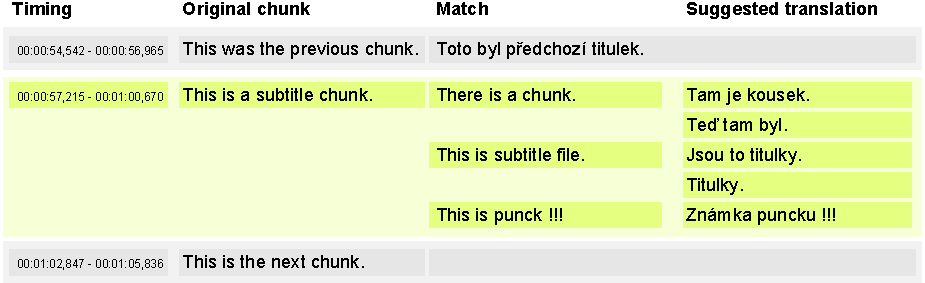
\includegraphics{./figures/original_strucutre.pdf}
\end{center}

\caption{Scheme of the originally intended structure of work with the translation memory. It reflects the original User Space structure and also schematically the original client design.}\label{fig:original_scheme}

\end{figure}

Very soon, we started to try to solve the video playback in the browser, which we expected to be a really challenging issue. We did some research about \emph{Adobe Flash} technology. We were also thinking about creating a hybrid solution -- an application wrapper with a web browser inside, capable to ensure the video playback for the inner web application.

We very soon had toy implementations of:

\begin{itemize}
\item a player using VLC plugin, to be incorporated into the web application

\item a player as a desktop Java application, showing the web application in a frame
\end{itemize}

\begin{figure}[h!]
	\centering
		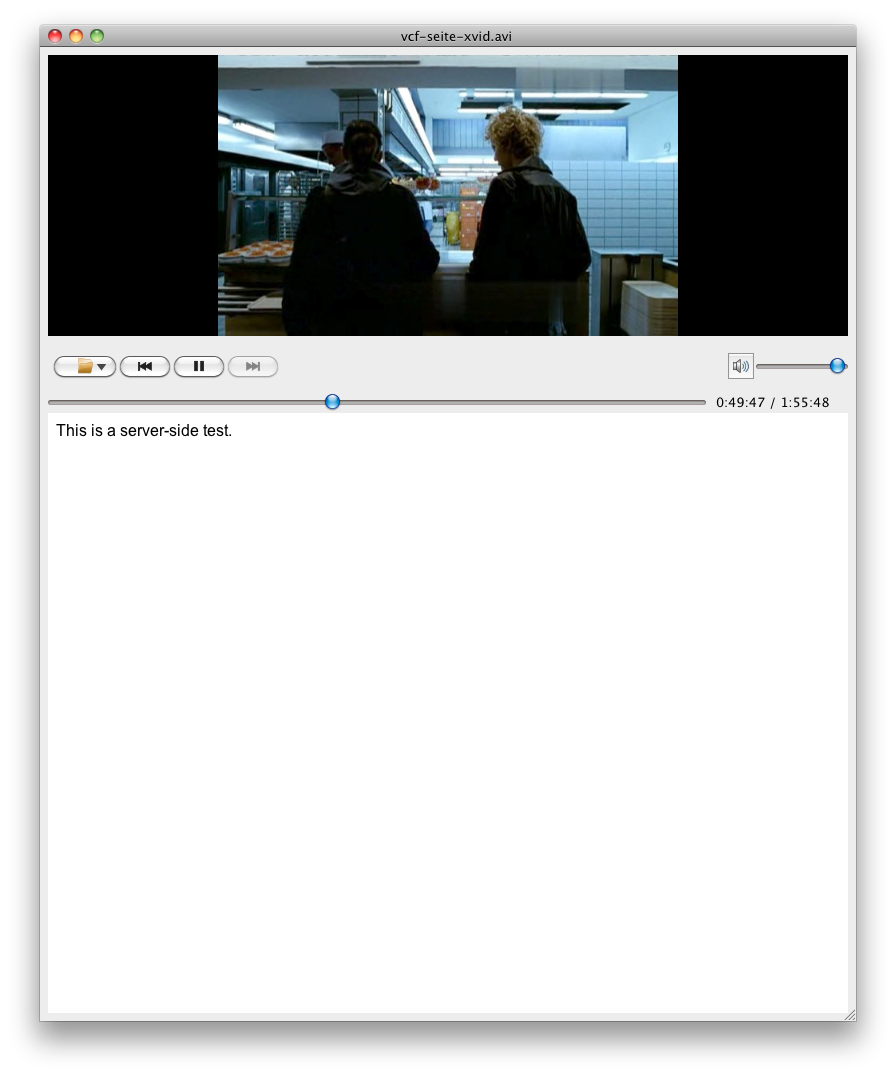
\includegraphics[width=7cm]{figures/desktop-app-player.png}
	\caption{Screenshot of Qt-based desktop application.}
	\label{fig:figures_desktop-app-player}
\end{figure}

We decided for the web application only version, with no desktop variant, because, observing the development trends, it seems to us that the present and future of applications is in web applications. The benefits are e.g.\ that the learning curve is typically better for a web application, where the user is already familiar with most of the controls and work patterns, installation is not required, so anyone can start using the application immediately, it is easy to use OpenID registration.

Still, there are disadvantages, especially the cross browser support issues, limited power, and larger bandwith consumption.
A GWT added advanatage is that the bandwith consumption is actually closer to that of a standalone desktop app, because the application itself is stored in one Javascript file, which is downloaded at the beginning (similar to installing a desktop application, but it is done transparently), and the rest of the client-server interaction is done through RPCs (basically the same way as it would be done in a desktop application).

\todo{player -- Karel should write something more about its development, the applet signing, etc.}

An issue we encountered in developing the player and were not able to combat completely is letting the user choose a media file and passing its full filesystem path to the player. We found out that although it is quite easy to load a whole file from disc into memory, only its filename is passed to Javascript instead of the full path for security reasons. We did a thorough search on the internet but found out that there is most probably no clean way around this restriction.

Ultimately we came up with 3 solutions, but none of them pleases us enough:

\begin{itemize}
\item the user inputs the full path as a string into an input box; works well but is not user-friendly (most users probably do not even know that such a thing as a filepath exists)

\item the user chooses the file in the file browser and then copies the file path from the browser inputbox into a textbox; this is probably even less userfriendly

\item a Java applet is loaded to choose the file as Java applets do not have such restrictions as Javascript, and then passes the path to the application; it seems to us too heavy-weight to create and load a whole applet only to get the file path, but it works quite well -- except for the users who do not have Java installed and working properly (we have also encountered an alternative using Flash for the same purpose, but we still prefer using Java to Flash)
\end{itemize}

We decided to use the third option, with the first option also available as a fallback for users who do not have Java running properly and thus cannot use the applet. \todo{we dont have that, right?}

\subsection{Introducing the shared classes}
\label{subsec:introducing_shared_classes}

After having implemented a very basic version of all three parts of the project, we decided it was time to start to solve the interoperability of individual parts in order to run a first snapshot of the application. This was happening approximately in March 2012.

At this stage we found out that we are not fully taking advantage of using the Java technologies for all parts of project and decided to totally redesign the User Space and Client parts.

Originally, we wanted to keep the traditional translation memory structure where each sentence can have several matches and these matches can have several translations in the memory, as is depicted in Figure~\ref{fig:original_scheme}. However, this scheme did not reflect much the way we worked with the data
%in the ???core???
in the Core
that time --
suitable matches were provided from the table of translation pairs based on indexes built over the table \todo{I dont undersatnd this sentence --RR}
and there were very few matches having multiple different translations in the data.
Also, the design of the GUI was a little bit confusing because the text of the matches was placed more prominently than the translation suggestions, despite the fact that the user is probably much more interested in the actual translation suggestions than in the matches. This lead to a modified scheme which is depicted in figure \ref{fig:new_scheme}.

\begin{figure}
\begin{center}
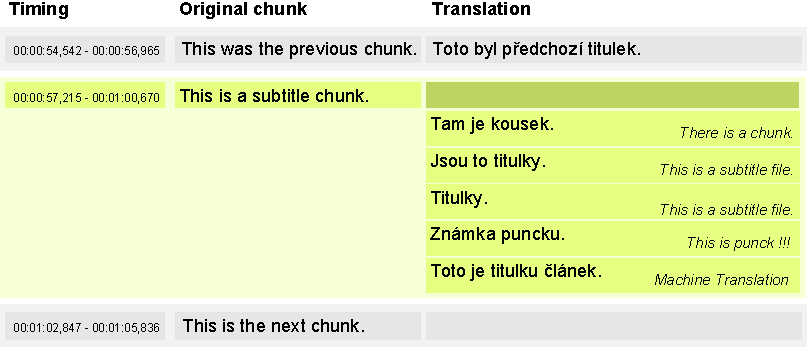
\includegraphics{./figures/current_strucutre.pdf}
\end{center}
\caption{Current scheme of the work with translation memory.}\label{fig:new_scheme}
\end{figure}

We agreed on the shared classes that all parts of the project should use. We more or less adopted the design of the classes from the core and started to use them in the whole project. This step required to re-implement the Scala classes in Java and to drop a lot of code that was already done in the User Space and the client. The design of the classes was almost the same as is described in \ref{sec:shared_structure}. \todo{but where is it?!}
\todo{hey, the ref is invalid since the section does not exist!}
From a later point of view, it appears to be an important decision to agree on the shared classes, which made the cooperation between the modules easier and less verbose. 

\todo{does this REALLY belong to subsec:introducing\_shared\_classes ?!?!?!?!}

We started the work on the project with the new design soon, which lead to a period of the biggest struggle with technologies. It took us almost two months to have the first running version of the application.

The very first version of the application was a page where it was only possible to upload a subtitle file and to do the translation, without any possibility to load an already saved subtitle document or download the result of the translation, without any sessions or users; it was just a page where you edit the subtitles (which later became the Translation Workspace).
At that time we used machine translation from the MyMemory service (which in fact wraps Google Translate), but there is a limited access per IP address and we soon began to reach the limit very frequently. It became obvious the we would have to change the source of machine translation. \todo{so we took Moses}

We also used API of IMDB.com to receive information about movies but the movie meta data was not used in the evaluation the matches at that time. (We had to switch to Freebase later because the IMDB service was discontinued.)

\subsection{The Main Development Phase}

It is hard to define the main development phase which is covered in the following paragraphs. It corresponds to the period from the beginning of March when the important design changes were made (see previous section \ref{subsec:introducing_shared_classes}) to approximately the middle of August when adding new features was stopped (see next section \ref{subsec:final_development}).

The section is divided to parts covering the issues we were dealing with and describes what we did in each area in those approximately five and half months.

\subsubsection{OpenID}
\label{subsubsec:openid}

Despite we wanted to implement OpenID support from the very beginning, we started with it approximately in May. We found two most frequently used Java libraries for OpenID and tried them. Those were \emph{JOpenID} and \emph{openid4java}.

\emph{JOpenID} seemed to be easier to use and also was much smaller as a dependency; on the other hand, when we run into some problems with using it, we found out that \emph{openid4java} is much more frequently discussed on the \emph{StackOverflow.com} forum and that there is a bigger chance that we would be able to find some advice for potential problems.

\emph{Openid4java} library is much bigger than then \emph{JOpenID} (it has megabytes whereas \emph{JOpenID} has tens of kilobytes) and supports not only logging in but also providing an OpenID endpoint service. When we found out that the problems with the libraries were because of wrongly set Maven dependencies, we turned back to \emph{JOpenID} library which is much easier to use.

At the end we decided to use \emph{JOpenID} library, and to support Google, Yahoo and Seznam accounts. The library contains Google and Yahoo by default. We decided to also add support for \emph{Seznam.cz} as the biggest Czech OpenID provider \todo{ref?}. Seznam provides the authentication data (we are particularly interested in the user name and email which we use in our application) in a different form than the other OpenID providers, therefore it was necessary to write our own parser of the authentication data ({\tt{cz.filmtit.userspace.login.SeznamData}}).

We do not support generic OpenID because the library does not support it. Anyway, after doing some research on the Czech developers forums, we concluded that just a very small percentage of users actually know what OpenID is; therefore, allowing to login via the Google and Seznam accounts is hopefully enough.

The support for OpenID was finished in July, the parser for the authentication data from Seznam was added at the beginning of August.

A question to solve was what to do when the user logs in through OpenID for the first time. We were thinking about requiring an explicit registration from the user in such case, but then decided that we probably do not need any more data than we already get from the OpenID provider. Therefore, we decided to register the user transparently in such situation.
However, because it can happen that e.g. the OpenID provider is temporarily unavailable, ceases to provide his services or that the user closes his account at the provider, we decided to offer the user a possibility to log in to his account even without the OpenID. For that reason, we create a full account for such user, generating a username and password and sending these to his e-mail address (which usually can be acquired from the OpenID provider).

Because the generated username is not only used as a backup way of authentication but is also displayed to the user in the top right corner of the application, we wanted to generate one that the user would recognize as being his. At first, we simply took the username part of his e-mail address (i.e. the part before the @ sign) and used it directly. However, this eventually leads to collisions, so we had to implement something more sophiticated.

The most primitive solution was iteratively trying to append numbers to the username if it was already taken, starting with 1, and checking whether such username was available. This was then improved to starting not at 1 but at the number of occurences of a username with the wanted username as a prefix, thus heuristically skipping the other usernames probably created in a similar way (and probably a few more just to be sure). And finally, we changed the iterative step from a simple increment to multiplication by 2, breaking any possibly remaining long sequences of already existing usernames.

Moreover, the user has the possibility to change his username and/or password on the Settings page.

\subsubsection{Chunk Splitting}

\todo{people who did that should add the text !!!}

ideas:

keep as it is, i.e. one timing = one chunk ... too long, too arbitrary

split into sentences, joining already split sentences together ... very hard (probably impossible) to do reliably, would miss the advantage of subtitle files for alignment

now: keep already existing splits, split on dialogue boundaries, slit on sentence boundaries (+ clean away irrelevant characters)

... easy enough to do reliably (SOME NUMBER of errors)

... arbitrary but not so much as the first solution

... length is reasonable

Important: to do the splitting in the same way when creating the database and when processing the user subtitles.
Therefore: a shared Parser class which is compiled both into java bytecode and used in impoting, and into Javascript and used in GUI

\subsubsection{Chunk Time Format}

\todo{please check whether this is true}

% Originally, we simply used the time strings acquired from the subtitle files to represent the timing, as we only displayed them to the user.
% 
% This was sufficient at the beginning; however, once we began fitting the media player to the actual subtitle lines, we needed to parse the time strings and convert them to a one-ineteger representation of time in miliseconds (we also needed that for editing the timing, which came later).

After a period of repesenting the time simply as a string, we created a class, SrtTime, that represents the time in the SRT format as a set of four integers (the SRT format of time is ``hh:mm:ss,ttt'' -- hours:minutes:seconds,miliseconds).
%\footnote{a milisecond is a thousandth of a second, thus the usage of the letter ``t'' to represent it; alternatively, knowing that the word ``second'' stands for the second diminuation of the hour, you can think of the milisecond as a third diminuation of the hour, also leading to the letter ``t''}).
We then decided to move all time handling logic into this class, so that we can ensure the correctness and consistency of the timing throughout the application.
The class provides various constructors, getters and setters for all formats we need, also performing validity checks.
% (one string, a set of strings, a set of integers, one integer being the time in miliseconds). It also implements cloning, comparison and subtraction.

At first, we decided to use the SRT format only for the sake of simplicity.
It was thought to be only a temporary state, with a plan to add SUB format support later. However, we eventually found out that not only is the SRT time format easier to use (it is not necessary to know the Frames-Per-Second property of the movie file),
but also approximately 98\% of subtitles on the internet appear to be in the SRT format \todo{please correct the number and add some source !!!}.
Thus, we decided to discontinue support for the SUB format and only support SRT (the only major difference between these formats is actually the format of the time).

\subsubsection{Chunk Annotations}

\todo{people who did that should add the text !!!}

named entities = first reason for annotations

chunk splitting by dashes denoting individual dialogue speekers: dashes need to be removed for translation suggestions generating because they are irrelevat but need be kept for correct rendering of text -> annotations extended to contain dialogue dashes

need to identify the newlines (irrelevant for translation suggestions but necessary to render the subtitles properly) -> annotations extended for newlines

subtitle formatting for bold, italic, underline etc. Original idea: extended the annotations again (easy to do). Then: too much trouble, expecially for GUI. Decision: just strip off these, do not support that. Reasoning: used very little, no formal specification so has various formats, often the players do not support the formatting properly so we want to discourage the users from using the formatting

chunk now has a set of methods to get and set the chunk and annotations correctly, using the notion of FORMS. The forms used are:

database form: the text as stored in the subtitle file, only cleaned -- formatting stripped off (bold, italic etc.), non-printable characters turned into spaces, multiple spaces replaced by one space only... The newlines are stored as PIPE characters.

surface form + annotations: the surface form is the text to be used to generate the translation suggestions, without dashes and with newline turned into spaces

GUI form: HTML form to be displayed in GUI, i.e. newlines turned into BR tags

text form: to be used in textarea -- with dashes, newlines as BACKSHLASH N characters

\subsubsection{Logging}

In US and core: easy, we use (whatever we use) \todo{pease specify}
and print the logs to the standard output (which is typically redirected to a textfile).

However, logging in the GUI is much more tricky, as there is no ``standard output'' or ``console'' to write the logs to.

Actually, it should be noted here that when using the GWT Development Mode, there is a console available to the programmer, where e.g. exceptions can be inspected, and GWT even provides the GWT.log() method to explicitely log messages to the Development Console -- which was found out only later. However, we still find it more useful to be able to see the debug messages even when not running the Development Mode; moreover, some of the members of our team were unable to run the application in the Development Mode successfully.

The preliminary logging solutions included various implementations of the common practice of ``debug prints'' (which is often used by programmers if the support for effective debugging is little or none) --
%In our situation, the debug prints were typically ensured by window alerts; we also tried changing the page title or statusbar for a less aggressive way of showing debug prints. Still, none of these solutions can be used in a larger scale.
window alerts, changing the page title or the statusbar text.

The solution we soon took for the development phase was to add a debug window at the bottom of each page, and a static method Gui.log() that prints the log messages into that window.
This proved to be very useful: once we added a large enough amount of logging, we were able to locate many issues that were appearing only using the contents of this window, often also guessing their causes as well.

The debug window served its purpose well; however, it obviously could not be left to appear in the final version of application.
It even would not be as useful, since the errors that would appear in a window of a browser of an external user (i.e. not a member of our team) cannot be accessed from our side.
However, there still might be errors that we would like to track and fix in future. This is a natural feature of most existing applications, and instead of denying it, we believe it is much better to try to count with it and prepare for it -- in our case, to find a way to make the GUI logs available to us on the server side instead of the cilent side.

The ultimate solution we took is what we call ``remote logging''. Important messages are now sent to the server through an RPC, where they are both included into the server log and saved into the database for possible future use (together with the userID if possible).
The minimal level of a meesage to be sent to the server can be set (debug, info, warn, error).
We first wanted to simply replace the implementation of Gui.log() by the remote logging; however, the original logging method did not have log levels, and the ammount of log messages generated was far too large to send all of them through the RPC. So, the remote logging must be used explicitely; it is now used especially for unexpected exceptions and RPCs.

We were not able to catch unexpected exceptions at first, as a GWT application does not have any ``main'' method where we could add a try-catch block to catch exceptions not caught by the inner components (which are the unexpected exceptions).
However, we eventually found out that GWT provides the static method GWT.setUncaughtExceptionHandler(), which enables the programmer to add a handler to catch all unexpected exceptions, which would otherwise escape to the browser.
Therefore, we implemented an ``exception catcher'' that, when given an exception, gets its stacktrace as a string, and logs it together with its name.

An interesting feature of GWT is that it provides stacktraces with filenames and line numbers from the Java source code, making it possible to use the stacktraces quite comfortably to debug the application.
Unfortunately, they are not always completely reliable, as some information might be missing in some situations.
Still, logging the exceptions with their stacktraces proved to be extremely useful in debugging the GUI.

Later we also encountered ``umbrella exceptions'' -- an umbrella exception is an exception thrown when multiple exceptions have occured at once, and contains all of them. Its message and stacktrace are not useful at all because they only cover the creation and throwing of the umbrella exception itself, but do not reveal anything about the inner exceptions. Fortunately, it does contain these details in other fields, and the exception catcher was successfully extended to show information about the inner exceptions in case an umbrella exception is thrown.

It is to be noted that in case of exceptions comming through the RPCs, the stacktraces are hardly ever useful as they do not contain information about the server classes where they originated.

\subsubsection{Implementing the RPCs}

From the start it was obvious to us that we want to use a well-estabilished method to implement the Remode Procedure Calls.
We noted in the specification that we would probably use JSON for the message serialization.
Fortunately, GWT does provide a ready-to-use Remote Service implementation, where the programmer only has to define the set of RPCs as an interface, implement the interface on the server side, and invoke an RPC on the client side by implementing the GWT AsyncCallback interface.
Everything else is handled automatically by GWT (which, as a matter of fact, does actually serialize the messages to JSON internally).
% Our first idea was to directly send and receive JSON messages because they have a format of a Javascript object, so we thought that this would be easy and efficient to implement in GWT (it is possible to read the object from string into memore simply using Javascript eval() function). However, there are three facts that we later found out that made us change our decision.
% The first one is that, although it is possible to directly use eval() function to convert the JSON message into the in-memory object representation, this practice is not recommended for security reasons (any Javascript code can be injected and it would be directly executed with no constraints). Therefore, the recommended practice is to use a JSON parser, which validates the JSON object before calling eval().
% A related issue is that although GWT sometimes does use JSON internally, it does not provide a JSON parser to be used by the programmer, so one has to use an additional library.
% And finally, we found out that GWT already implements a mechanism to send RPCs (in which, as a matter of fact, the messages are actually serialized to JSON).

The type of an RPC parameter or return value can be any GWT-compilable type. Because this type must be known both to the server and to the client, we use only primitive types and shared classes SEE XXX. Each class sendable through GWT RPC mechanism must implement the GWT IsSerializable interface (which is only a marker, i.e. it does not have any abstract methods) and a parameter-less constructor; this also holds for the checked exceptions, which are technically only a special type of a return value.

Because of Javascript and browser limitations, the RPC mechanism of GWT only allows asynchronous calls from client to server. This suited our needs often, but we had to go around these limits in some situations. Quite often we need the RPC to be synchronous and blocking, e.g. in logging in or changing user settings. In such situations, the page or dialog is ``deactivated'' on invoking the RPC (all active components are disabled -- e.g. the textboxes are read-only, the buttons do not respond to clicks), a reference to the page or dialog is passed to the class invoking the RPC, and when the RPC returns, the page or dialog is ``reactivated'', either with a success message or an error message, depending on the result of the RPC.

In one case, we would need an opposite direction RPC, i.e. the server to invoke the RPC on the client. This is when authenticating the user through OpenID, where we have to perform the authentiation in a new window -- the new window then receives the result of the authentication, but it cannot be easily passed directly into the opener window. Here we decided to use active polling -- the opener window regularly invokes the GetSessionID RPC, which returns null if the authentication process has not yet finished, this being a signal for the GUI to continue polling. To link together the opener window and the authentication window, a unique authID, generated by the User Space, is used.
% Originally it was created by the GUI and sent to User Space, but we soon found this to be inappropriate so the User Space now generates the authID.

\subsubsection{Failed RPC Requests Handling}

% Originally, all the RPC requests followed the barebone AsyncCallback interface, where the request is sent to the server, and onSuccess() or onFailure() method of the callback are called once it returns, depending on the result. The default implementation of onFailure() was to display the error message to the user, the idea behind being that it is eiher a mistake of the user that he should be informed about, or a mistake of the server which he should be informed about as well. This was sufficient for most of the cases; however, it became clear to us that time to time, the requests fail for various reasons beyond our reach (usually temporary network problems), where the default behavior of simply informing the user (and usually throwing away the data he generated for the request) is often not welcome.

We decided that our general error handling strategy should be to try to solve all problems without user interaction, and to inform the user only about user-generated errors (such as incorrect SRT file format or session timeout) or critical errors (such as permanent loss of connection to server).

The first thing was to turn the calls into objects,\footnote{This is very similar to the XXX design pattern. %I found it but I forgot the name.
} so that they store their parameters and can be called again on failure. We also created a generic superclass for them, Callable, filled with necessary boilerplate code and methods performing the default actions, to be overridden if necessary.

We identified the response that we usually get in case of network problems (it is a StatusCodeException with the status code 0). The problems can be temporary or permanent; in case of temporary problems, the default response of showing an error message was found to be highly inappropriate, as it would suffice only to resend the call. Therefore, we introduced retrying the call for three more times in such case with short delays, before showing an error message to the user.

The retrial of calls has proven to be an efficient way to deal with problems, so we decided to extend it to all types of failures. However, in case of non-network errors, we soon found out that retrying the calls does not make sense in some situations; so we decided to keep the retrial as a default action which can be overridden in the exteding classes.

We also added a timeout for each request after which the request is regarded as lost and is retried. Such situation is not at all typical, but we need to count with it to prevent the user from ``starvation'' (the user can always escape from any state by refreshing the page in the browser, but this can lead to an uncontrolled local data loss or even to objects being left in an inconsistent state -- such as a document without content).

\subsubsection{Sending Translation Results}

At first, the translation suggestions from the Translation Memory were requested and sent for each chunk individually. This had the theoretical advantage that the user received each of the translation suggestins as soon as possible. However, we found the overhead of the RPC calls to be unreasonable. Not only was the overall time necessary to load all the suggestions too long, but also a typical browser was unable to handle such a large number of requests and usually froze for long periods of time, often unfreezing only after all of the suggestions arrived.

A simple solution seemed to be sending all of the chunks for translation in one request. However, such a request can take several minutes to complete, and we still wanted to keep the nice property of the application showing the suggestions as soon as possible at least for the first lines -- so that the user can start the translation immediately. Thus, we decided to send the request in batches, starting with a small size of the batch for the beginning of the file and gradually increasing the batch size.

The first way to do that was an exponential increase, where each batch contains twice as many chunks as the previous one, starting with a batch of size one. This proved to solve the aforementioned problem of browser freezing; however, another problem arose. As the batch sizes grew larger and larger, the later requests often took several tens of seconds or even minutes to complete. Meanwhile, the user would often navigate away from the Translation Workspace, rendering the translation suggestions, including the currently being processed ones, obsolete. This was of course detected in GUI and the suggestions were thrown away on arrival, but still it meant that the server was working in vain for some time, possibly resulting in an unnecessarily slower responsiveness to other users (and even to the very same user as well).

We introduced two further solutions. The first and simple one was limiting the size of the batch to 64 chunks (which typically only take about ??? seconds to process), so that the amount of useless work could not grow too large. The second one, which took us some time to think up and implement, was to stop the translation suggestions from being generated on the server, by issuing a StopTranslationResults request. (This breaks the typical model of procesing the queries, where once a query is sent, its processing is not influenced by queries that arrive later.)

The two major issues with the StopTranslationResults request were:

- to interrupt the suggestions generating which is already in process (which is done in parallel for the chunks in the batch, making this even harder).

- to identify what to stop and what to let continue.

The first idea was to mark the whole document as closed, and to check this when generating the suggestions. However, this would cause problems if the same document was immediately reopened by the user, and even larger problems if the user already had the document opened twice -- this can easily happen by mistake, the logical reaction of the user is then to close one of the Translation Workspaces, and then he would stop receiving suggestions even in the other opened Workspace. Thus, we then decided to create an identifier for each Translation Workspace instance and to bind the StopTranslationResults request to this identifier. However, we soon found out that this would require a lot of overhead only to handle this probably not very common situation, so we dropped that idea as well.

Finally, we decided for a compromise solution between those two. The StopTranslationResults request is now bound to individual chunks, which now have an added boolean field isActive. This field is set to true when the GetTranslationResults request arrives to the server, for each of the chunks on the request. The StopTranslationResults request contains a list of the chunks which translations should be stopped. On arrival of that request, User Space simply sets the isActive field to false -- because User Space and Core share the same memory and because only references to the chunks are passed around, this change is visible in core even though the chunks have already been sent for translation. The necessary overhead is minimal, and there is no "false alarm" in the typical case. The only unsolved case is the situation where the same batch of chunks are sent for translation at the same time from two different instances of Trabslation Workspace with the same document opened, and then one of these Workspaces is closed, causing the suggestions generation to stop even for the batch from the other Workspace. Although this situation is unlikely and non-critical (the suggestions would be missing only for this one batch, the later batches would be translated correctly), we still offer a general solution by repeating all request on failure (unless it is obvious that the failure will reoccur).

\subsubsection{User Management}

At the very beginning the only the GUI was basically only the translation workspace. It was possible to translate a subtitle file in the application, the changes were reflected in the database, anyway it was not possible neither to get them in the application when the web application was reloaded neither to export the subtitles.

We considered the user management to be just a minor technical issue. Anyway, to enable to reach the intended architecture of the User Space -- mostly that most of the calls should be resolved in the Session objects -- we introduced a simple fake login in April (you could log as any user using password "guest").

We stared to implement the OpenID login support in May (see section \ref{subsubsec:openid}). When we met some technical difficulties. We decided to implement first our own registration and login.

Because our own experience that requiring a registration from a web service often prevent us from using it we decided to make the registration as easy as possible. We have no constraints on user name (except for non-emptiness) and very little constraints on password (only it must be at least characters long).

We think the most important feature of a password is for the user to remember it, we leave the assessment of the strength to the user. The password strength constraints are often rather arbitrary and many classes of strong passwords do not pass them, it is hard to develop a reasonable strength measure. E.g. a whole sentence, a "passphrase", is a very strong password; however, it usually does not pass measures requiring use of specific classes of characters. And vice versa, a password using very unusual characters (e.g. Czech letters with diacritic signs) can be impossible to break even if it is quite short, because the attacker simply does not try out such characters that are uncommon in passwords; still it often does not pass typical minimum password length constraints.

Moreover, we are not forced to pay much attention to the security of the application - it does not contain any sensitive data whose compromising would pose a threat to the users of the application and the benefit to the attacker successfully breaking into a user account is close to none.

We allow the user to work in multiple browser tabs or windows, provided it is the same session (i.e. has the same SessionID), because we believe it is natural to work on multiple translations at once, to have the Document List opened to see the translation progres, etc. The user himself is responsible for having the same document opened multiple times, which is not expected behavior and so changes to the document in one Translation Workspace are not projected into the other Workspace until reload.

However, we decided to disallow one user having multiple sessions at one time, as we believe that this is neither expected nor required behavior, and could potentially confuse the user. We believe that such a state is usually caused by a mistake, e.g. user A forgetting to log out on PC 1, then moving to PC 2, and at the same time user B using the application on PC 1 under user A's account by mistake.
We do not support multiple users collaborating on one subtitle file.

If user registers through OpenID, we have to assign a user name to him (the unique OpenID identifier we get is typically a long hash, which does not look like a nice user name), see section \ref{subsubsec:gui_openid}. Because the user name is at least partly generated, the user might not like it. Therefore, we offer each user the possibility to change the user name (provided that the one he chooses is free). The user name is only used to authenticate the user (if not using OpenID login) and is displayed in the top right corner in the application; the internal unique identifier of a user is his user id, an integer assigned to each user on registration that never changes.

\subsubsection{GUI Look and Feel}

After using default GWT look, we decided to use Twitter Bootstrap -- good decision, looks nice and provides additional widgets.

\begin{figure}
\begin{center}
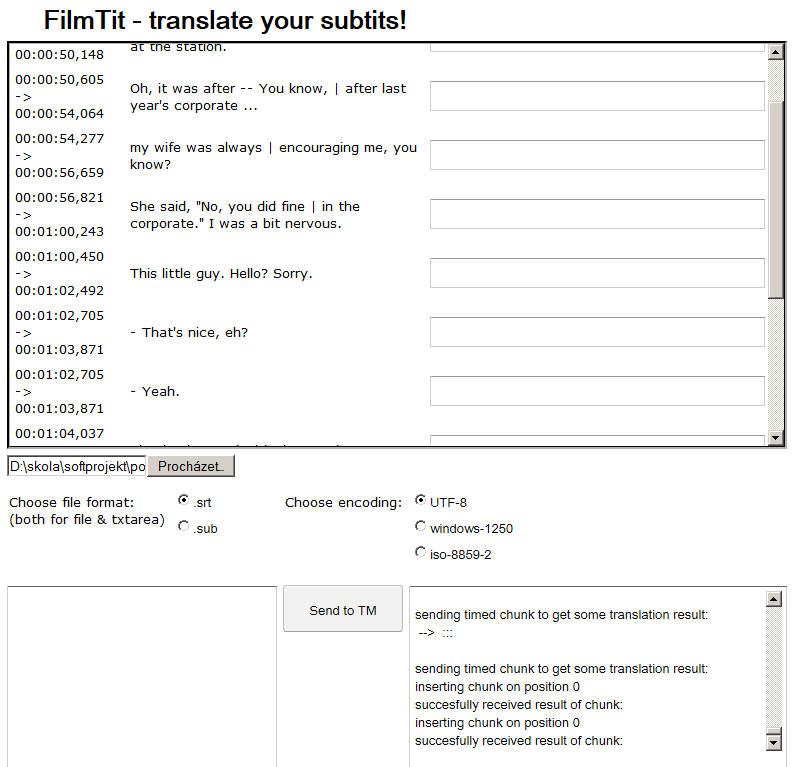
\includegraphics[scale=0.5]{figures/old_screenshot.png}
\end{center}
\caption{Design of the Translation Workspace before starting to use the Twitter Bootstrap}
\label{fig:before_bootstrap}
\end{figure}

Trying to be user friendly

\begin{itemize}
\item expected behavior
\item as litle controls as possible
%- can be controlled by mouse %(except for typing)
\item TranslationWorkspace can be controlled both by mouse and by keyboard, as the user is expected to spend most of the time in Translation Workspace by typing, and the need to switch between the mouse and the keyboard would decrease his efficiency
\item other pages controlled only by mouse, which feels natural enough; a typical user spends most of the time in Translation Workspace, therefore having to use the mouse on the other pages is not expected to be an efficiency problem
\end{itemize}

changing data .. idea: it should be possible to change anything if there is not a strong reason why not
\begin{itemize}
\item change document title, movie title... by clicking on it (seems natural, added a tooltip)

\item change timing or source text: we think that this is not usually required so it is under a double click to prevent unwanted activation (and a tooltip again)

\item we offer the user the possibility to change the source text because if there is an error, the suggestions might be incorrect (the suggestions are regenerated on changing the source)

\item we do not offer deleting chunks because this would be difficult to implement properly in GUI; however, the default behavior is not to export the untranslated chunks, so not translating a chunk is roughly equivalent to deleting it

\item we do not allow to change the source subtitle file (this would actually mean deleting the whole old document and creating a new one, probably only keeping the title -- so we leave this for the user to do himself); however, smaller edits can be done directly in TW
\end{itemize}

\subsubsection{Subtitle Formats}

first support for SRT and SUB

more and more problems with SUB

internal format of time is SRT

finally decided to support only SRT

- AFAIK 99\% of subtitles are in SRT

- easier to process (e.g. changing the timing), easier to sync to the player

(We also support exporting the subtitles in plain text format, i.e. only the text without timing information.)

\subsubsection{GUI Pages}

We started having one page only, the Translation Workspace, which was sufficient for development of the application for several months. Later we added the Document  Creator page as the default one, which replaced itself by the Translation Workspace once a document was created, and this was sufficient for some more time. However, we eventually could not avoid adding more pages and the need to explicitely handle multiple pages became obvious.

We immediately found out a week point of GWT here: it has nearly no native support for multiple pages. This was quite a surprising issue to us, since in any other web development technology or framework that we know, creating a new page and switchng pages are really simple tasks. GWT, however, observes the idea of having one HTML file and one Javascript file only that handle everything. (It is technically possible to create multiple pages by creating multiple GWT projects, each corresponding to one page, but this is not recommended for many good reasons.)

The GWT way of switching pages is by replacing the contents of the Root Panel (which represents the visible part of a page), or any other Panel placed within the Root Panel (which we decided to use so that some elements, such as the menu, are present on all pages). The switching is done without reloading, simply by creating an instance of the new page and directly setting it as the contents of the panel (without any convenience functions for that to our knowledge).

All the pages have the same URL by default, but GWT offers the History class for changing the URL and reacting to changes to URL (however, it is not linked to page switching by design -- this remains for each programmer to do by himself). There are also Hyperlink widgets, which represent a link to a different page, with the default action being changing the URL and invoking the appropriate handler (a ValueChangeHandler).
The URL contains an anchor with the name of the page (e.g. \#DocumentCreator or \#WelcomeScreen), and the History class is able to provide the name of the anchor to the user and to invoke the ValueChangeHandler when the URL changes.

We decided to use the History class and Hyperlinks to implement the menu and page switching. We create a PageHandler class which implements the ValueChangeHandler -- it turns the anchor string into a value of Page enum, checks whther the requested page can be loaded (especially based on the user log in / log out state) and loads the appropriate page. It also provides public methods to other parts of GUI so that they can switch pages, modifying the URL at the same time (so that the browser refresh works as expected).

However, we encountered one issue with the Hyperlinks: the ValueChangeHandler is invoked only if the value of URL changes, which means that if the user clicks a menu link which points to the page loaded (e.g. while creating a document, the user decides to restart and clicks the document creator link), the handler is not invoked. As this behavior is hard-coded into the Hyperlink class, we had to abandon the Hyperlinks and used NavLinks instead (a simple link with no default interaction with the History), with click handlers invoking the ValueChangeHandler.

When reviewing the resulting code, we found out that the History class and the ValueChangeHandler do not provide any benefit to us any more, so we removed them completely. Only then did we find out that the History class can also correctly handle the browser's forward/backward button behavior, so we readded it, but it is only used for that purpose now.

Another issue encountered was the fact that passing the page name as an anchor name is not always convenient and sometimes is not possible at all. If the page requires some additional parameters -- such as the password change page, where the user can change his password based on a link sent to his mailbox, containing a temporary token and the username as parameters -- the resulting address looks odd (e.g. http://filmtit.cz/?username=a\&token=df5ds3f\#ChangePassword). Moreover, the OpenID validation mechanism we used requires URL of a return page as a parameter, to which it adds parameters containing information about the validation process, but it is only able to add the parameters at the end of the address, resulting in an incorrect URL. For such cases, we decided to offer an alternative way of specifying the oage to be loaded in the URL by setting the page parameter (e.g. http://filmtit.cz/?page=ChangePassword\&username=a\&token=df5ds3f).

This solution finally proved to offer all features required.

We also had a discussion about the expected page to be loaded in various situations. E.g., if the user is in Translation Workspace and logs out, the URL page parameter stayed on Translation Workspace by default, although Welcome Screen is displayed instead because a logged out user does not have access to Translation Workspace. If he then logged back in without switching the page, the document he had opened before logging out was reopened again.
Eventually, the behavior was modified so that the URL is always changed to Welcome Page when the user explicitely logs out, but the URL is not modified if the user is logged out automatically, typically because his Session ID expires. Reasoning: if he was logged out implicitely, it is probable that he did not want that and woud like to continue with his work as soon as possible. However, if he logged out explicitely, he probably finished his work and expects the application to be ``closed'', i.e. not remembering the last stae of his work.

(TODO: tidy a little, I dont like that subsubsection very much...)

\subsubsection{User Space Robustness}

User Space started as nice but not robust -- it was not prepared to receiving erroneous data, it had concurrency issues especially when there were multiple users performing similar actions simultaneously, etc. This was probably caused by the fact that User Space was developed several months before it was first used, due to delays in GUI development.

TODO: When we tried it out, we were getting tons of errors, so some checks were added and locks were introduced, so now it works nicely.

\todo{probably remove this subsub}

\subsubsection{Handling Parsing Errors}

% At first, the subtitle files were expected to be in the correct format -- no explicit checks were performed and if an error was encountered, the file was rejected.
% The SrtTime class was then added 

We found that since many subtitle files are partly or fully generated by people, and probably also because the SRT format has no official specification, errors in the files are very common. Rejecting even the files with only minor errors (such as a surplus or missing newline, or an incorrect time format which we check thoroughly) showed to be unnecessarily strict, as typically most of the file is correct and the number of errors is small.

We decided to introduce heuristics to decide whether to reject the whole file: if the number of recoverable errors is lower than 10, the erroneous parts are skipped and the rest of the file is parsed.

\todo{Karel to nejak upravoval, tak at si to sem napise}

% However, this lead to also rejecting
% We were improving the situation gradually, eventually creating a new exception class, InvalidDocumentFormatException, which is thrown by the parser, with a 
% Also, as a preliminary check, we refuse any file which is larger than 500 kB. We introduced this check because it is very fast and efficient.

\subsubsection{Offline Mode}
\label{ip:subsubsec:offline}

At first, our intention was to make the whole application able to run offline. However, it was not a priority and was not even part of the official specification.
Eventually, we decided that the only part that has to be able to work offline is the Translation Workspace, as doing the translation itself is the most time-consuming part of the whole process for a user. We believe that the user can prepare everything while online, wait until the translation suggestions are loaded, and then spend some time offline translating the document.

We also decided to require for the application to stay open while the user goes offline, as it would be difficult to reload the aplication offline
-- e.g. the whole application would have to be stored offline, which we wanted to avoid in the first place by designing FilmTit as a web application.
However, it is obvious that the data created by the user in Offline Mode must be stored locally even if the application is closed.
Thus, only storing setUserTranslation calls and invoking them once the user goes back online turned out to be sufficient.

% (this is only a discussion explaining why not to support more, I would leave it out)
%
% Creating documents and exporting documents: not possible in Offline Mode.
% Settings: does not make much sense in Offline mode.
%
% Only thing that IMHO could actually be useful is preloading multiple documents, so that user can got to doc list and back again and translate multiple documents, not only the opened one.
% Would have to preload suggestions -- would have to change the way they are handled since now they are not stored permanently anywhere, are always regenerated on opening the TW.
% The question which documents to preload -- all of them? Too unefficient. Only the ones that user chooses? Yes, but he has to be able to choose them in a user-friendly way. Probably simplest: store the documents that the user opens. However, there is then little difference between the targetted state and the current state: the only difference is that now the user must open multiple tabs and leave them opened, while in the proposed state he could open them one after another and work on them in one tab only (although StopTranslationResults would probably have to be modified as well so that the user does not have to leave the TW open and wait for all of the suggestions to load). \todo{nevim jak se anglicky rekne ze to je malo muziky za hodne penez}

\paragraph{Technology}

We decided to use the HTML5 Local Storage, which is similar to the well-known cookies mechanism from which it evolved.
Like Cookies, the stored object has two ``useful'' string fields, the name (or ``key'') and the contents (or ``value'').
However, the Local Storage has several advantages over cookies:

\begin{itemize}
\item The objects are not sent to the browser on loading the page but are stored and retrieved on request. This would actually be a disadvantage if we wanted to interact with the storage from server side; however, in our case, being only able to handle the objects from within Javascript is an advantage.
\item The size limit both for individual objects and for the total ammount of data stored is larger.
\item Instead of setting expiry time, the programmer simply decides whether the objects should be stored temporarily (for a browser session) or permanently (which is our case).
\item The API is cleaner.
\end{itemize}

Still, thanks to the similarity of Local Storage to cookies, it would be quite easy to implement a fallback for browsers without Local Storage support using cookies. We decided not to do that because, as far as we know, most browsers installed on users\' computers nowadays do support Local Storage. However, we might add this feature in future if there is a need for it.

\paragraph{Serialization}
Because the necessary serialization is special -- we need to serialize into a set of two strings, the key and the value, with the key being a unique yet intelligible identifier of the object -- we decided to implement our own serialization, defined by the Storable interface which is described in Section~\ref{gui:subsubsec:storable}.
However, we encountered an issue with Java support for interfaces: Java does not support neither constructors nor static methods in interfaces.
Still we need to use the one or the other for deserialization (or a hack, such as using an empty constructor and then loading the data into the empty object, which would enable us to define the method in the interface, but would break several good programming practices otherwise and therefore we decided not to use it).
The Java reasoning is understandable -- one could specify the one or the other, but they could never be invoked through the interface without specifying the implementing class, so there is no point in including them.
We agree that including methods that can never be invoked is strange. However, we would understand if these methods were removed from the interface during compilation; still, it would be helpful if the classes implementing the interface would be automatically checked for implementation of such methods, both in IDE and at compile time.

% We decided to define a static factory method fromKeyValuePair that all Storable classes must implement; however, it has to be commented out in the source code of the Storable interface, as well as the ``@Override'' annotation in the implementation classes. Still, we prefer to keep these in the code to make our point.

\paragraph{Extendability}
Although currently only one class, SetUserTranslation, can be stored in Offline Mode, the Offline Mode support is desinged to be easily extendable if we decide to store other data in Local Storage as well.
To add support for storing another class in the Local Storage, the class would have to implement the five methods defined by the Storable interface (especially the serialization and deserialization methods, the other three are trivial to implement). Apart from that, only some handling logic would have to be added or modified, such as reaction to the GUI being probably offline, etc.
(In the current implementation, it is silently supposed that the stored objects are RPCs that should be invoked on comming back online. However, this is reflected mainly in the way the Offline Mode procedures communicate with the user, which would be easy to change if nescessary.)

\paragraph{Object Identification}
When some objects are stored in the Local Storage, they can only be accessed through the Local Storage interface, which is flat and does not support any advanced structures -- the programmer can only get the number of all of the objects in the storage, iterate over their keys, and retrieve a value of an object based on its key. (Plus setting and deleting the objects of course.)
Thus, we had to find our own way to identify the objects correctly, so that we correctly inform the user about objects he has stored (not objects that other users stored) and correctly deserialize them and perform any actions required -- this means that not only the object contents but also an identifier of its class and of the current user have to be included. We found two possible solutions:

\begin{itemize}

\item store a special object or objects in the storage, describing the other objects:

\begin{itemize}
\item efficient retrieval of the description of the contents of the storage
\item could simulate a simple file-system with a tree structure of files and folders
\item the object key can be any uniquely generated string
\item not reliable as the user can interrupt the application at any time and can also change the values stored by the application
\item could still be used as a non-authoritative cache
\end{itemize}

\item each object contains all necessary information in its key

\begin{itemize}
\item simpler to implement
\item very little danger of data corruption
\item keeps the flat structure
\item the object key must include all important information to identify the object
\item all object keys must be loaded to know the contents of the storage (but it takes at most a few seconds in a typical case)
\end{itemize}

\end{itemize}

We decided to use the second approach, which we believe should be always used to prevent data corruption; however, we think that it would be beneficial to also implement and add the first approach as an additional layer of abstraction above the individual objects.

% \item decided that this might be good to add in future but there seems to be no need at the moment
% \item started with the ``key fields'' of the objects (document id and chunk index in case of SetUserTranslation)
% \item then also added the class name to make it extendable (although it has not been extended)
% \item then added username because there might be various FilmTit users using the same browser
% \item and eventually changed username into user ID because now the user can change his username

\subsubsection{Hibernate Issues}

Before starting the project, nobody of us had any experience with an object-relation mapping library for Java. Initially we were also thinking about not using such a library and using the \emph{JDBC} connection directly -- that was the option we chose for the translation memory core where we work only with a few tables with simple relations. Concerning the User Space, where we expected much more complicated structure, we thought that using an object-relation mapping would be more beneficial and decided to use one.
% AN object-relation mapping!!! for X's sake, it begins with an "[o]", how can you say "a object..."?! or is it because you say [vobjekt]? :-)

After doing a little research on the Internet, we found out that Hibernate seems to be the most frequently used library for object relation mapping and decided to use it. There were more than 20,000 discussions on \emph{stackoverflow.com} which gave us hope that solution for any problems we might have could be easily found on the Internet. 

Details of the mapping itself can be found in Section~\ref{subsec:database_mapping}, the structure of the mapped database is in Figure~\ref{fig:em_of_us}. Here we will focus on the database mapping from the development perspective.

Because we started with Hibernate version 3, all properties we wanted to make persistent had to provide getters and setters. The requirement to have a getter and a setter for each property may sound as violating the encapsulation feature of the Object Oriented Programming, but in fact the getters and setters can be private (as Hibernate can still access them via reflection). Each class also must have a parameter-less constructor, but it also can be private.

New versions of Hibernate allow to use the fields of the classes directly, but since the mapped classes are usually wrappers of the shared classes, most of the fields are only accessed through getters and setters in the rest of the application, so we just use getters and setters for all the properties. Despite we ended up using Hibernate version 4.1.0, we are quite conservative in terms of using its features and keep all the mapping in separate XML files despite it can be done by annotations directly in the source file and do not access fields directly, but always use getters and setters.
% "the fields are not directly accessible from the mapped class" ?!?!?! WTF ?!?!?! you can make a class which cannot access its own fields???

The previously mentioned requirements of Hibernate were very often sources of minor bugs -- mostly forgetting to add a private setter (which soon lead to exceptions and was easy to find), or forgetting to add a new property into the mapping (which did not lead to immediately observable errors, as this only had the result of the property not being persistent; moreover, when a new property was added, it was usually not covered in tests at that time, so it typically took some time to find the bug.)

Another problem was that although Hibernate can adjust the database scheme to the mapping if the mapping changes, it was often not able to change it in a proper way and it was necessary to drop the User Space tables in the database and let Hibernate create them from scratch. This of course always caused loss of the data we tested the application on. More importantly, this means that it would be very hard to change the mapping in the application once it is released -- it would probably require managing the database scheme changes partly or fully manually.

% haha, I would just keep that a secret so that they let us defend it :-D
% During debugging of one bug (it was happening that the same translation results was appearing in the database with different database IDs) it appeared how useful is to use the database constraints. If we had had it before this bug would have been found right away and it would not take so much time to find it. After this experience we added constrains everywhere where it was possible.

\subsubsection{Media Source}

was IMDB, is Freebase now

https problems

adding the "null" option

\todo{this is a todo for Jo I am afraid}

% not very interesting I am afraid
%
% \subsubsection{GUI Refactoring}
% 
% TODO: have that here or not??? Yes!
% 
% Started as 1 class (GUI.java) which grew and grew.
% 
% The RPCs handling moved to a separate class.
% 
% Subgestbox class.
% 
% Introduced UiBinder for designing the GUI.
% 
% The notion of pages, each having its own java class and an UiBinder template.
% 
% Introducing the PageHandler.
% 
% The RPCs turned into individual classes in cz.filmtit.client.callables
% 
% The pages moved to cz.filmtit.client.pages and all are displayed simply by creating the class.
% 
% The notion of Dialogs, residing in cz.filmtit.client.dialogs, with Dialog being the superclass (peviously just hardcoded somewhere).
% 
% The sbgetsbox gets its own subpackage.
% 
% Gui made static

\subsubsection{Subgestboxes}

One of the most important features of the application's user interface is the behaviour of the actual translation workspace, particularly the text-boxes where user writes their translations and which provide the pop-up suggestions from the translation memory. Since the functional requirements for these boxes were gradually refined throughout the development process, their implementation also underwent several stages of evolution. However, their class' name, SubgestBox, remained from the early stages, implying the idea of a box offering suggestions for subtitles.

\paragraph{SuggestBox?}
First, we were thinking about the GWT pre-implemented SuggestBox, probably with some slight adjustments. However, we realized that with our specialized demands on its behaviour and appearance (especially formatting the suggestion items, later also multi-line input ability), this class would not be sufficient and we would probably need to extend one of the more general classes in the inheritance chain. Still, we have drawn some inspiration from the SuggestBox class implementation; for example, using a PopupPanel to show the suggestions proved to be quite an elegant solution.

\paragraph{Base widget}
For some time, we were using a common TextBox with the suggestions pop-up extension, switching after a while to a TextArea to offer multi-line input. But since we also needed some text formatting inside the box (e.g. for the named entities' annotation highlighting or for the user formatting, such as italicized text) which could not be added by a simple extension to the TextArea, we have once again switched the base class, this last time to the RichTextArea.
(Eventually, none of the formatting is supported in the current version, but we decided to keep the RichTextArea implementation to have an easy way of possibly adding such functionality in future.)

\paragraph{Fake and real}
The RichTextArea, being based on the IFrame HTML element, provided all the functionality we have requested (although some of it is not as simply accessible as we expected), but there was yet another problem with it. Having one IFrame for each chunk on the page, i.e. hundreds of them for an average movie, turned out to be quite a significant performance problem -- the browser often became irresponsive. In the end, we have solved this issue by distinguishing so-called ``fake'' and ``real'' SubgestBoxes; the former being simple TextAreas and displayed by default in the translation workspace, on focus transforming into the latter, the real IFrame-based SubgestBoxes with all the functionality.

\paragraph{Focus handling}
With all the complexity of the SubgestBoxes switching and suggestion selection (and initially, also because of the asynchronicity of the suggestions arrivals), we could not rely on the default focus handling mechanisms of the browser. If we wanted to provide a keyboard-only control for the user when translating (which is often a key to an effective translation speed), we had to devise our own mechanism of the focus traversal between the SubgestBoxes and/or the suggestion pop-ups. This issue, seemingly simple, proved to be quite complex to cover all the implications and, in the end, some cross-browser inconsistencies (not captured by GWT) had to be solved manually by pieces of browser-dependent code. As usual, particularly one of the hints found on the web-forums proved to be very useful, namely the suggestion of always wrapping the setFocus method in a ScheduleDeferred command.

\paragraph{Automatic scrolling}
In order to relieve the user of manual scrolling when going through the SubgestBoxes in the translation workspace and avoid the whole-page auto-scroll when the focus is gone outside the page, we used the ScrollPanel's method ensureVisible to automatically scroll each focused SubgestBox to a fixed place in the browser window (currently it is approximately 2/5 of the window's height), later rewritten more generally to be used independently on any ScrollPanel. However, this feature also partly clashed with the suggestions popping up, so there had to be also lots of tuning and experimenting with the command deferring.

\paragraph{Endlines}
Since it was our intention to also allow multi-line inputs in the SubgestBox (reflecting for example the cases of translations being sometimes significantly longer than the original chunk), we had to cope with an issue of RichTextArea of inconsistent newline handling in different browsers, expressed by Table~\ref{implprocess:RichTextAreaNewlines}. Our solution was to keep this different formatting while the user is translating, convert it to our unified format (i.e. every newline represented by the \verb=\n= character, stripping of beginning and trailing newlines and shortening sequences of them into one) when the translations are sent to be saved in the userspace, and to show the newlines as \verb=<br />= when loaded from the userspace again. This behaves quite well in all of the tested browsers and does not interfere much with the idea of the RichTextArea's HTML-based system.

\begin{table}[h]
\begin{center}
\begin{tabular}{|l|l|l|}
\hline
browser & getText()             & getHTML() \\
\hline
Firefox & \verb=first linesecond line= & \verb=first line<br>second line<br><br>= \\
\hline
Chrome  & \verb=first line=            & \verb=<div>first line</div><div>second line</div><div><br></div>= \\
        & \verb=second line=           & \\ 
\hline
Safari  & \verb=first line=            & \verb=first line<div>second line</div><div><br></div>= \\
        & \verb=second line=           & \\
\hline
IE9     & \verb=first line=            & \verb=<p>first line</p><p>second line</p><p>&nbsp;</p>= \\
        & \verb=second line=           & \\
\hline
Opera   & \verb=first linesecond line= & \verb=<p>first line</p><p>second= line</p><p><br></p> \\
\hline
\end{tabular}
\end{center}
\caption{Table capturing different handling of newlines across browsers, showing the return values of the RichTextArea's getText() and getHTML() methods. In all the cases, the text entered was ``first line[enter pressed]second line[enter pressed]''.}\label{implprocess:RichTextAreaNewlines}
\end{table}

\paragraph{Automatic resizing}
With the possibility of allowing multi-line inputs, we had to manage the size adjustments of the input area. And since the RichTextArea itself does not have any pre-implemented tools for this purpose, we again had to devise our own.
Because of the difficulties with the newline handling (see above), we have abandoned the direction of counting lines manually and built the mechanism on getting the scrollHeight property of the input area. Then, auto-growing of the SubgestBox is relatively easy, but auto-shrinking turned out to be more difficult, because the scrollHeight does not decrease. So a simple trick of setting the size to one line at the beginning of each adjustments was employed and fortunately did not significantly affect the performance.

\paragraph{Popup widget}
The suggestion pop-up widget has not come through so many fundamental changes, rather some styling or minor adjustments. Since its introduction, the CellList class was used as a base for this widget, only initially the cell rendering was implemented by hand as a simple table. Later, for the sake of clarity and convenience, we also switched this rendering to the UiBinder template-based structure, namely SuggestionPopupStructure. This way, its structure is more readable, more easily stylable and even supposedly faster in its displaying.

\paragraph{Fake vs. real styling}
When introducing the ``fake'' SubgestBox, as opposed to the ``real'' one, we were also facing an issue of making them visually as similar as possible, not to bother the user with this implementation workaround. But since we were overriding GWT and GWT-Bootstrap styling, we had to be very specific in the CSS class identification to address and change the SubgestBox' visual appearance. Unfortunately, one of the side-effects of this was for example a need to change the CSS identification when the basic widget for the ``fake'' SubgestBox changed from a TextBox to a TextArea.

\subsubsection{Subtitles Export}

When implementing the subtitles export feature, we encountered an unexpected issue:
GWT cannot create a new file, neither on server (beacause it is all Javascript) nor on the user\'s computer (because of security restrictions).

We found several possbile solutions:

\begin{itemize}

\item export the subtitles into a textarea
\begin{itemize}
\item the easiest to implement
\item not what a user expects
\item not easy to use for the user
\end{itemize}

\item send the exported subtitles to user\'s e-mail address
\begin{itemize}
\item quite easy to implement becase we already have implmented the e-mail sending
\item might be useful for some users
\item not what a user expects
\item can be hard to use for the user
\item might be added as a special feature but should not be the only or primary way
\end{itemize}

\item create a temporary file on the server and offer a download link to the user
\begin{itemize}
\item expected behavior from the user (file download using the browser)
\item reasonably reliable
\item reasonably easy to implement
\item should handle access rights in Jetty which is an added complication
\item creating temporary files is not very clean
\end{itemize}

\item create a new servlet (using JSP) for downloading the file
\begin{itemize}
\item expected behavior from the user (file download using the browser)
\item probably the cleanest possible solution
\item we were afraid that it would be too much extra work, but we realized that it was not so difficult
\end{itemize}

\end{itemize}

Eventually, we decided for the last option as the best one; therefore, the User Space actually consists of two servlets, one to handle RPCs and another for file download.

\subsubsection{Chunks Saving / Loading}

We originally decided that the subtitle file will be parsed in the GUI, 
to avoid unnecessary sending of the data from GUI to User Space and then back from User Space to GUI; parsing the file in User Space would also cause unnecessary load on the server.

Although we wanted to make everything as parallel as possible, we found out that we have to save all the chunks immediately after parsing so that they do not get lost; therefore, requesting the translation suggestions is only done after that, even though this means that the translation suggestions start arriving a little later.

To also enable editing the files, the Translation Workspace became the only page that has two constructors -- one receiving the text of a subtitle file to parse, and the other getting an already parsed document from the database.

\subsubsection{Login}

A requirement we had on the login functions was that they do not require reloading the page. This is because it might happen that the user\'s sessionID expires, which would lead to his last request being lost in case of realoding the page. However, not reloading the page enables us to resend the request once the user is logged back in.

This was easy to do in case of the Simple Login. In case of OpenID Login, it lead to a rather complicated procedure (see Section~\ref{subsubsec:gui:openid}), which requires opening a new window for the user to authenticate on the OpenID provider webpage.

\subsection{Final Development}
\label{subsec:final_development}

\todo{since when is it "final development"?}

Optimizations required: better to throw away translation pairs and generated every time user logs in

Found many technical issues: %e.g. necessary to be able to stop loading generating the suggestions on the server at the moment - DONE


We left
a lot issues which we considered to be only minor and technical
to the end of the development process;
naturally, many of them were eventually found to constitute a lot of intensive work.

We set the Feature Freeze to the 12$^\mathrm{th}$ August, 12 p.m.
% Feature Freeze is an existing term, it is not our invention! :-)
After the Feature Freeze, no new features were added to the project, and we started an intensive review of already existing code, debugging, and working on the documentation.

\section{Evaluating the Development Process}

One of the crucial decision for the project was the choice of technologies. Most of the technologies we used -- Maven, Scala, Hibernate, GWT -- were new to all of us and we also had not much experience with the other. Combining these technologies together was quite painful and would probably even for an experienced Java developer. Generally, we can say that the fact that we were not too much familiar with the technologies, we spent most of the time solving technical issues. There is quite a lot of research challenges, mostly in the fuzzy matching part, which had to remain untouched due to that.

On the other hand the choice of technologies appeared to be lucky that it probably saved a lot of work for us by the possibility to share implementation of class. Using the Scala language for the core also made the parallelization much easier.

Despite we spent quite a lot of time by the discussions how the structure of the project we didn't avoid a radical change of the design of the application 4 months after the project started. Nearly the whole User Space code had to be dropped and it was also necessary to totally remake the client components existing so far.

A bottleneck of the development process was also that not all of us were familiar with all of the technologies. It happened many times that somebody could not continue developing a particular part of the project and had to wait for an other team member to fix the issue even though it may have been just changing a single attribute in the Hibernate mapping.

During the whole time we had little problems that our development process is not as effective as we would imagine and it also difficult to find suitable communication platform. Despite we used see each other very often to discuss the project issues and had regular meetings, a working online communication was played a crucial role for us.

As a very first communication channel we established a mailing group at Google groups. All the notifications and comments from Github were redirected to that mailing group as well as results of Jenkins builds. Soon we started to receive dozens of Filmtit email every day and it started to be quite difficult the follow the conversations and find something in the conversation history.

Because of that we tried to use the Piratedpad\footnote{http://www.piratenpad.de/}. It is free a web-based collaborative real-time editor, allowing authors to simultaneously edit a text document, and see all of the participants' edits in real-time, with the ability to display each author's text in their own color. There is also a chat box in the sidebar to allow meta communication run by the German Pirate Party. We tried to keep there personal plans and ``todos'', bug reports. After some time it became quite messy and the mailing group became the main communication channel again. We were also solving a lot of issues bilaterally using various instant messaging systems.

In July, when the most intensive work on project started, we launched a Skype conference. It effectively replaced the personal meetings, which was much sought after as usually several members were out of Prague at a time, but fortunately they typically had internet connection.
It also helped to solve many issues instantly and efficiently.
However, it has a same disadvantage as email conversation -- it is difficult to easily find facts in the history -- but now with hundreds of messages every day to make things worse.
Fortunately, because almost every time there were at least some team members online, it was always possible to ask for a summary of previous discussions and we managed to keep all the team members informed about everything important.

Mid-August, however, there was a decline in using the Skype conference -- we found out that when all of the project members were online and the work on the project could have been expected to be very intensive, it often actually happened that very little work was done since most of the time was spent on discussions through Skype.
Another issue was that some members tended to use the conference simply for chatting about non-related matters, %including me of course --R
which later made it even harder or nearly impossible for the others to find important messages in the history.
We then started to send the most important messages through the e-mail conference again and, eventually, we mostly switched back to it.

\section{Possible Future Development}

There are many things to be improved, mostly in the graphical interface. It would be probably possible to add new features forever. If there ever would any newer version it would probably include support for more language pairs.

We would like to let project run for some and wait if it would find its community of users. If it would reach some success among the user, it would provide a lot of interesting data -- mostly about preferences of the users which translation suggestions are useful for them. Such information could be useful for developing new fuzzy matching techniques including some research challenges as finding matches to a part of sentence. Success among users would also mean a growing source of well structured data for statistical machine translation.